\documentclass[10pt]{article}         %% What type of document you're writing.
\usepackage{graphicx}
\usepackage{hyperref}
\usepackage[dvipsnames]{xcolor}

%%%%% Preamble

%% Packages to use

\usepackage{amsmath,amsfonts,amssymb}   %% AMS mathematics macros

%% Title Information.

\title{COMPANY Data Model}
\author{Adolfo Centeno}
%% \date{2 July 2004}           %% By default, LaTeX uses the current date

%%%%% The Document

\begin{document}

\maketitle

\begin{abstract}
This document implements the COMPANY Data Model.
\end{abstract}

\section{Data Model Description}

The COMPANY database keeps track of a company’s \textcolor{red}{employees}, \textcolor{red}{departments}, and \textcolor{red}{projects}



\begin{enumerate}

\item
  
The company is organized into departments. \\
Each department has a unique \textcolor{green}{name}, a unique \textcolor{green}{number}\\
and a particular employee who \textcolor{yellow}{manages} the department. 
We keep track of the \textcolor{green}{start date} when that employee began managing the department. \\
A department may have several \textcolor{green}{locations}


\item
A department \textcolor{yellow}{controls} a number of projects, each of which has a unique \textcolor{green}{name}, a unique \textcolor{green}{number}, and a single \textcolor{green}{location}

\item
The database will store each employee’s \textcolor{green}{name}, \textcolor{green}{Social Security number}, \textcolor{green}{address}, \textcolor{green}{salary}, \textcolor{green}{sex(gender)}, and \textcolor{green}{birth date}.\\ 
An employee \textcolor{yellow}{is assigned} to one department, but may \textcolor{yellow}{work} on several projects, which are not necessarily controlled by the same department. It is required to keep track of the current \textcolor{green}{number of hours per week} that an employee works on each project\\
**** as well as the direct \textcolor{yellow}{supervisor} of each employee (who is another employee). ****

\item
The database will keep track of the \textcolor{red}{dependents} of each employee for insurance purposes, including each dependent’s \textcolor{green}{first name}, \textcolor{green}{sex}, \textcolor{green}{birth date}, and \textcolor{green}{relationship} to the employee.

\end{enumerate}


\section{E-R Model}

COMPANY...

\begin{figure}[h]
     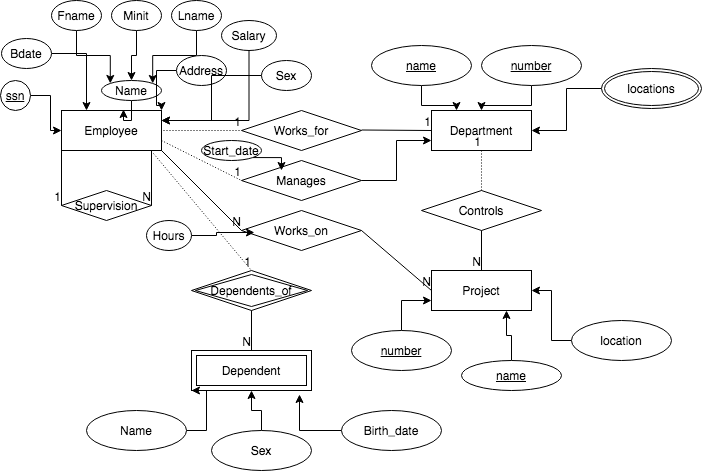
\includegraphics[scale=0.2]{er_company}
     \caption{COMPANY E-R Model}
\end{figure}
   
\section{Relational Model}
COMPANY Relational Model

\begin{figure}[h]
     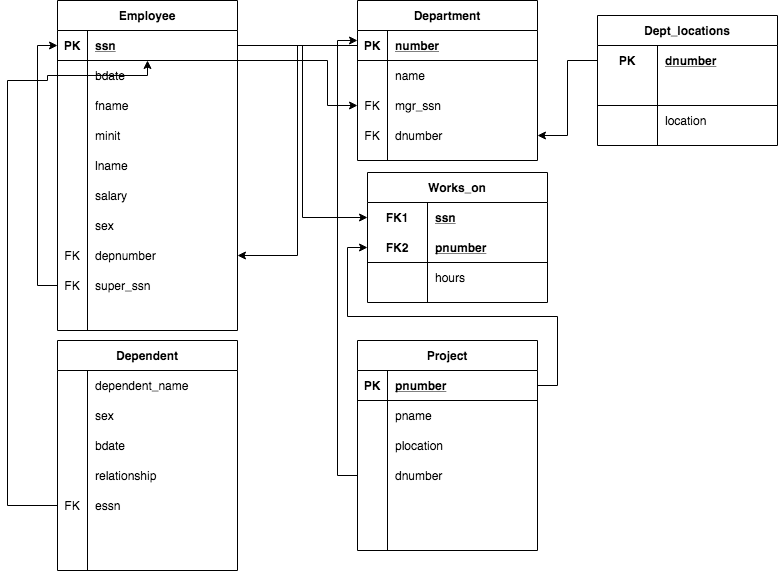
\includegraphics[scale=0.2]{relational_company}
     \caption{COMPANY Relational Model}
\end{figure}

\end{document}

